%************************************************
\chapter{The Presentation Tier}
\label{ch:presentation-tier}
%************************************************

\section{Introduction}

The presentation tier is located at the boundaries of the server side: it represents an entry point into the server. Its core responsibilities are to accept requests from clients, to figure out what business logic should be executed and finally to send responses in the appropriate format. 

The details of what happens in the presentation tier depends on type of client that sends the request: a thin client requesting web pages and a rich client requesting business data may involve different components on the server side. However, there are design patterns that apply in every situation. The objective of this chapter is to explore them. We will review the \ac{MVC}, the \ac{IoC} and the Pipes and Filters design patterns. After presenting them in generic terms, we will see how to concretely apply them with Java EE APIs and look at some code.

\section{The Model View Controller pattern}

\marginpar{MVC was first proposed in the context of GUI applications. In multi-tiered applications, MVC can mean different things. Rich clients and modern Javascript frameworks apply the traditional definition of the pattern. In the presentation tier, the pattern is applied quite differently. It is sometimes referred to as MVC2}

\ac{MVC} is one of the well-known design patterns and has been documented decades ago. It has its origin in the development of graphical user interfaces for desktop applications. The goal of the pattern is to clearly separate responsibilities between three software components. This leads to code that is easier to write, understand and maintain. In many software engineering courses and textbooks, the implementation of \ac{MVC} is illustrated with \ac{GUI} toolkits like Swing or Java FX. 

In the context of multi-tiered applications, be aware that \ac{MVC} can take different shapes and may be applied in different tiers. In the case of rich clients, \ac{MVC} takes its original form and is purely in the user interface domain. If you decide to use a client-side Javascript framework, such as Angular or React, you will be exposed to client-side \ac{MVC}. In the case of thin clients, \ac{MVC} is implemented on the server side, in the presentation tier. This changes quite a few things as the implementation does not involve a UI toolkit. In this chapter, we only consider the second situation. In other words, we describe a variation of the \ac{MVC} design pattern that operates on the server side. The key question is then to understand the relationship between the pattern components and the HTTP request-reply model.

\clearpage
\subsection{Description of the pattern}

The pattern involves the following participants:

\begin{itemize}
\item the \emph{model} is an object, or a graph of objects, that the user is interested in. Let's imagine that the user is accessing a product catalog: the model would be a List of Product objects, with properties such as Price and Description and with linked objects such as a List of Reviews or a Photo. Always keep in mind that you are manipulating graphs of objects: they need memory and bandwidth.
\item the \emph{view} is a component that produces a representation of the model. In the previous example, it could be a component that generates an HTML page with embedded images and hyperlinks. The view is generated on the server side, transferred to the client side, where it is finally rendered by a browser. In some cases, the representation is meant to be consumed by a human (e.g. HTML page or PNG image). In other cases, it is meant to be processed by a software agent (e.g. and XML or JSON payload).
\item the \emph{controller} is a component that reacts to user actions, is exposed to the details of the HTTP protocol and coordinates the work between the other components. In the case of thin web applications, whenever the user is taking an action (log in, access a product page, add a product in the shopping cart, send a message), he clicks on a link or a button, which causes the browser to send an HTTP request to the server. Every HTTP request is an event that represents a user action. It is comparable to a mouse event or a key event in a UI toolkit. When the server receives an HTTP request, it delegates its processing to the appropriate controller. The controller then has to extract information from the request (from the URL, the query string and/or the headers). The controller then decides how to generate a model and to ask a view to generate a representation of this model. Finally, the controller has to send the representation back to the client. At this stage, it is once again exposed to the details of the HTTP protocol.
\item the \emph{service} is a fourth component that is not strictly mandatory, but that is used very often to keep the code of the controllers small. In theory, a controller could create the model itself: by doing some sort of computation, by looking up information in a data store, etc. In practice, the controller will very often delegate this task to a service. In other words, it will handle the situation like this: ``Based on what I have seen in the URL and query string, I decide that Service A can handle the user action and generate a model for me. I also decide that View 1 can generate a representation of the model. I am going to coordinate the work between these two helpers.''
\end{itemize}

Figure \ref{fig:client-tier} shows the sequence of events for a typical user interaction round trip.
\begin{enumerate}
\item The user is visiting an online shop and is on a page that displays a list of products. For each product, there is a picture, a description, a price and an hyperlink entitled "Show details". The user has found an interesting product and clicks on the hyperlink. This where we start our exploration of the \ac{MVC} pattern.
\item The browser sends an HTTP request to the server. The method is \texttt{GET} and the URL is something like \url{http://shop.com/productsController?productId=4224&action=showDetails}. You can think of the HTTP request as an event, just like you would have a mouse event or a button even in a GUI toolkit.
\item On the server side, the HTTP request is routed to a component, which is the Controller in our pattern. Depending on the language and platform, the Controller might be an object or a function.
\item The Controller is lazy and tries to do as little as possible. Its first job is to figure out what other components can help him. Firstly, by looking at the attributes of the HTTP request (the URL, the query string, etc.), it will decide which business service can handle the request. It then calls the business service.
\item The Service does its job, which usually means getting some data, applying some business rules and computing a response. The response from the Service to the Controller is the Model in the pattern. It is usually an object or a graph of objects.
\item When the controller has received the Model, it looks for another helper: the View. Again, the controller is responsible to decide which of the available views can generate a representation of the Model. Usually, it looks at the HTTP headers sent by the client: the \texttt{Accept} header might indicate if the client prefers HTML or JSON. The Controller must have a way to pass the Model to the View, and to has the View to handle the last part of the processing. This depends on the platform and we will see the Java EE approach later in this chapter, with some code examples.
\item The last step is for the View to do the rendering and to prepare the response, which sent to the client.
\end{enumerate}

\begin{figure}[]
	\centering
    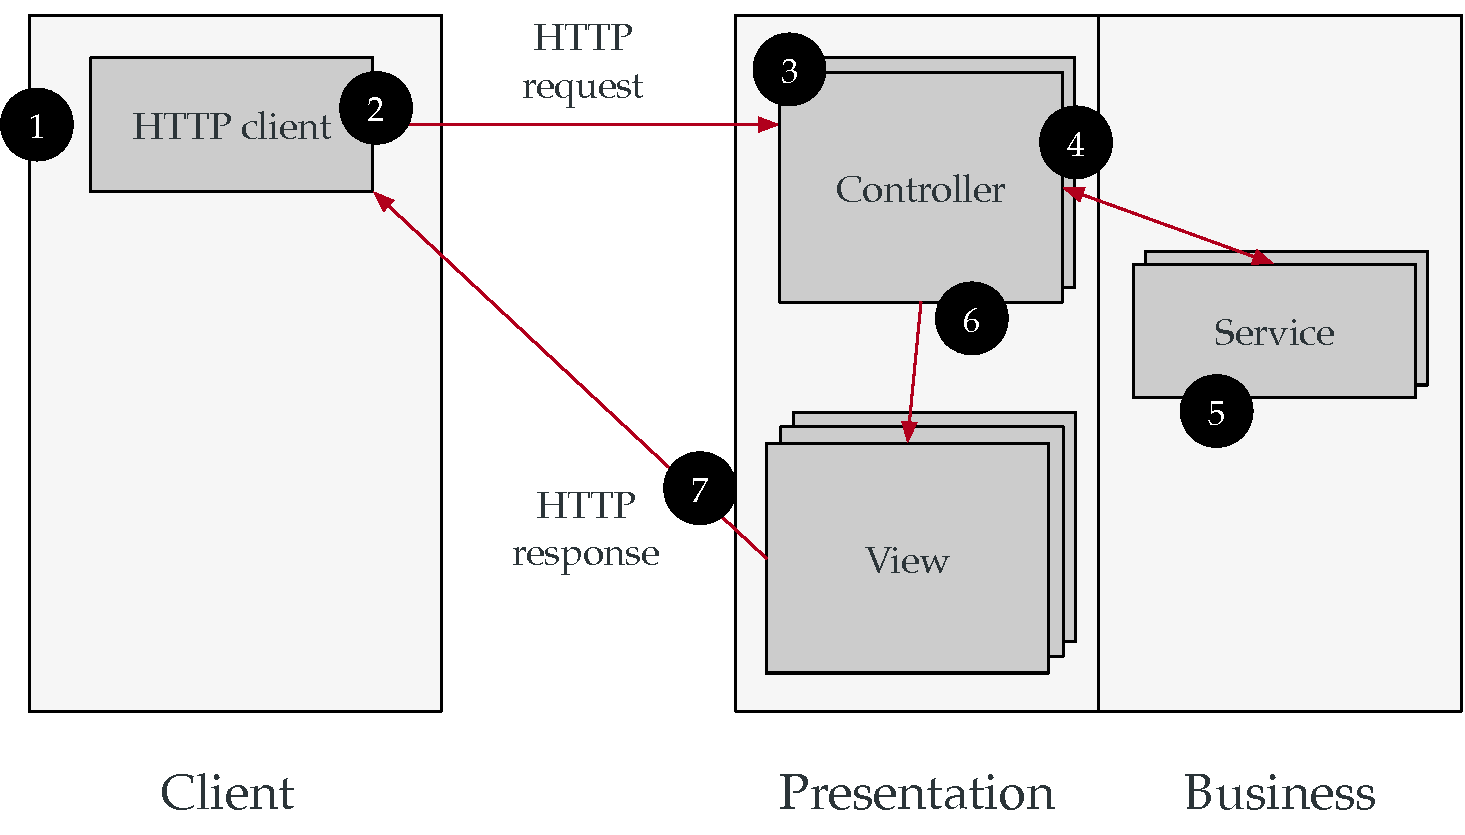
\includegraphics[width=1.0\linewidth]{Figures/MVC.pdf}
	\caption{The MVC design pattern in the presentation tier}
  \label{fig:mvc-in-presentation-tier}
\end{figure}

\subsection{Applying MVC in Java EE}

Let us know see how we can concretely implement the \ac{MVC} pattern with Java EE. For that purpose, we introduce two \ac{JSR}: the Servlet API and the \ac{JSP} API. 

A servlet is a Java object that implements a few methods, which are invoked when an HTTP request has been sent by a client. The responsibility of the servlet is to analyze the request (it has access to the URI, the HTTP headers, the body, etc.) and to prepare a response. A simple example is provided in Listing \ref{lst:quoteServlet}. 

\lstset{
	style=amt,
	language=Java,
	caption={A simple HTTP servlet},
	label={lst:quoteServlet},
}
\vspace{10pt}
\begin{minipage}{\linewidth}
\begin{lstlisting}[frame=single]
@WebServlet("/quote")
public class QuoteServlet extends HttpServlet {
  public void doGet(HttpServletRequest request, HttpServletResponse response) throws IOException {
    response.getWriter().println("<html>In cauda venenum.</html>");
  }
}
\end{lstlisting}
\end{minipage}

Let us review the code line by line:

\begin{itemize}
\item On line 1, the \texttt{@WebServlet} annotation is an instruction given to the application server. It is a way for the developer to state that when an incoming HTTP request targets the \texttt{/quote} URL, then the application server should forward it to this servlet. As we will see later, using this annotation is an alternative to the \texttt{web.xml} deployment descriptor.
\item On line 2, the developer creates a class by extending the \texttt{HttpServlet} abstract class, which is defined in the Servlet specification. The specification includes a Javadoc documentation for this class and its methods.
\item On line 3, the developer implements a method that will be invoked by the application server when the method in the incoming HTTP request is \emph{GET} (as opposed to \emph{POST}, \emph{PUT}, \emph{DELETE}, \emph{PATCH}, etc.).
\item The \texttt{doGet} method has two parameters. The \texttt{request} parameter is an object that represents a complete HTTP request. The \texttt{HttpServletRequest} class is also defined in the Servlet API specification. It provides getter methods to access the request method, URI, headers, etc. The \texttt{response} parameter represents the HTTP response. The developer uses this object to prepare the response sent to the client.
\item On line 4, the developer obtains a \texttt{PrintWriter} object and produces HTML markup that will be sent in the HTTP response body. The developer might also have added headers to the request. He might also have used an \texttt{OuputStream} object to send binary data to the client.
\end{itemize}

This is the simplest example to demonstrate how to build dynamic web applications in Java. But be aware that this example does not follow the \ac{MVC} pattern. The servlet is at the same time the Controller, the View and the Service (and for this reason, there is no real Model). Mixing HTML markup with Java code is a code smell. It is not rare to observe this in legacy applications and when it is the case, the maintenance is generally very painful.

\marginpar{Behind the scenes, the application server translates every \ac{JSP} template into Java source code, which it then compiles. The source code is actually a subclass of \texttt{HttpServlet}.}

Let us improve the code and introduce a View. For that purpose, we will use the \ac{JSP} technology. Historically, JSP was created a couple of years after the Servlet API. The technology provided a standard way to implement dynamic web pages and has been used extensively. It has evolved a lot over the years and many features have bean added either directly in its specification, or in companion \ac{JSR}s. Today, JSP is still supported by Java EE application servers and is a perfectly viable choice for building web applications. However, the technology has disappeared from official Java EE tutorials and seems to have lost traction with open source communities. Two factors can explain the situation:

\marginpar{\ac{JSP} has disappeared from the official Java EE tutorial. The last version that presents the technology and gives example is \href{https://docs.oracle.com/javaee/5/tutorial/doc/}{the Java EE 5 Tutorial.}}

\begin{itemize}
\item In 2004, the \ac{JSF} API was proposed as an alternative to JSP. The goal was to provide a solution for building component-based user interfaces, on the server side. This was a great idea, but it proved very hard to do. From our own experience, we can say that building web applications with \ac{JSF} was complex and time consuming. We moved away from the technology before it reached version 2.0, so things might have changed. Even if that is the case, we rarely see new projects adopt this technology, because the trend is now to build rich web clients. Hence, it is the surprising that the official Java EE guidelines put a very strong emphasis on \ac{JSF} and have even stopped presenting \ac{JSP}, a simpler and practical solution. Of course, if \ac{JSF} was widely adopted, it would be benefit certified Java EE application server vendors. The reason is that providing a \ac{JSF} implementation is mandatory for a fully compliant application server, but it is not for projects like Apache Tomcat.
\item At the same time, non-standard alternatives to \ac{JSP} have been provided by open source projects. \ac{JSP} is essentially a templating technology, and so are projects such as Thymeleaf, FreeMarker or Velocity. Frameworks that have been developed on top of Java EE, and in particular the very popular Spring MVC, do support \ac{JSP}, but often start by presenting other template engines.
\end{itemize}

Let us now how Java Server Pages look like and how they can be used in combination with servlets. The repository \href{https://github.com/SoftEng-HEIGVD/Teaching-HEIGVD-AMT-MVC-simple-example}{SoftEng-HEIGVD/Teaching-HEIGVD-AMT-MVC-simple-example}, hosted in GitHub, contains the code that we review here. Instructions for running the code with IntelliJ IDEA are provided in the repository \texttt{README.md} file.

\lstset{
	caption={Structure of the simple MVC project},
	label={lst:quotesProjectStructure}
}
\vspace{10pt}
\begin{minipage}{\linewidth}
\begin{lstlisting}[frame=single]
src/main
src/main/webapp
src/main/webapp/index.jsp
src/main/webapp/WEB-INF
src/main/webapp/WEB-INF/web.xml
src/main/webapp/WEB-INF/pages
src/main/webapp/WEB-INF/pages/view.jsp
src/main/java
src/main/java/ch
src/main/java/ch/heigvd
src/main/java/ch/heigvd/amt
src/main/java/ch/heigvd/amt/mvcsimple
src/main/java/ch/heigvd/amt/mvcsimple/business
src/main/java/ch/heigvd/amt/mvcsimple/business/QuoteGenerator.java
src/main/java/ch/heigvd/amt/mvcsimple/model
src/main/java/ch/heigvd/amt/mvcsimple/model/Quote.java
src/main/java/ch/heigvd/amt/mvcsimple/presentation
src/main/java/ch/heigvd/amt/mvcsimple/presentation/QuoteServlet.java
\end{lstlisting}
\end{minipage}

The structure of the project source files is shown in Listing \ref{lst:quotesProjectStructure}. Here is a description of the different packages and files:

\begin{itemize}
\item line 12: we use a namespace for the project: \texttt{ch.heivd.amt.mvcsimple}.
\item lines 17, 13, 6 and 15: we organize our classes based on the tiers of the architecture. We have controllers in the \texttt{presentation} package and services in the \texttt{business} package. We have views in the \texttt{pages} directory. The \texttt{model} package contains the classes that encapsulate business data and are used across tiers.
\item line 16: the Quote class is the \emph{model} in the application.
\item line 7: the view.jsp \ac{JSP} is the \emph{view} in the application.
\item line 18: the \texttt{QuoteServlet} class is the \emph{controller} in the application.
\item line 4: \texttt{WEB-INF} is a special directory and is present in every \texttt{.war} file.
\item line 5: \texttt{web.xml} is a \emph{deployment descriptor}. It describes the web application and is used by the application server at deployment time. In older versions of Java EE, the deployment descriptor was mandatory for all applications. Over time, the same information can be given to the application server via \emph{annotations} in the code. \emph{Warning}: the \texttt{web.xml} indicates the version of the Servlet API used by the application. Using an old version (e.g. by copying old examples found on the Web) may cause hard to debug problems.
\item line 6: the pages directory is located inside the \texttt{WEB-INF} directory. This is a security best practices. The Servlet specification states that it is not possible to access resources directly (i.e. it is not possible to type a URL in the browser to access them). The only way to reach them is to go via a controller. 
\end{itemize}

Now that we have seen the structure of the project, let us look at the code of the model (Listing\ref{lst:quotesProjectModel}), the controller (Listing\ref{lst:quotesProjectController}) and the view (Listing\ref{lst:quotesProjectView}).

\lstset{
	caption={The model class},
	label={lst:quotesProjectModel}
}
\vspace{10pt}
\begin{minipage}{\linewidth}
\begin{lstlisting}[frame=single]
package ch.heigvd.amt.mvcsimple.model;

public class Quote {

    private String author;
    private String citation;

    public Quote(String author, String citation) {
        this.author = author;
        this.citation = citation;
    }

    public String getAuthor() {
        return author;
    }

    public String getCitation() {
        return citation;
    }

}
\end{lstlisting}
\end{minipage}

Here are some comments about the \texttt{Quote} model class:

\begin{itemize}
\item lines 13 and 17: these two methods are often called getters, because they are used to get the value of an object property. The convention is to name these methods \texttt{getXXX()}, where \texttt{XXX} is the name of the property. Using this convention is not only a good practice that makes the code uniform and easy to read. It enables some of the magic that happens behind the scenes, because it facilitates dynamic code invocation. We will see a first simple example when we get to the code of the \ac{JSP} tempate. When we present the notion of \ac{ORM} later in the book, we will also explore the underlying mechanisms in more details. 
\item line 8: observe that the constructor allows us to define the state of the model object and that we did not implement any setter method. This is a good practice, when we want to work with immutable objects.
\end{itemize}

\lstset{
	caption={The controller class},
	label={lst:quotesProjectController}
}
\vspace{10pt}
\begin{minipage}{\linewidth}
\begin{lstlisting}[frame=single]
package ch.heigvd.amt.mvcsimple.presentation;

import ch.heigvd.amt.mvcsimple.business.QuoteGenerator;
import ch.heigvd.amt.mvcsimple.model.Quote;

import javax.servlet.ServletConfig;
import javax.servlet.ServletException;
import java.io.IOException;
import java.util.List;

public class QuoteServlet extends javax.servlet.http.HttpServlet {

    private QuoteGenerator service; // we will see later how to replace this with dependency injection

    @Override
    public void init(ServletConfig config) throws ServletException {
        super.init(config);
        service = new QuoteGenerator();
    }

    protected void doGet(javax.servlet.http.HttpServletRequest request, javax.servlet.http.HttpServletResponse response) throws javax.servlet.ServletException, IOException {
        List<Quote> model = service.generateQuotes();
        request.setAttribute("quotes", model);
        request.getRequestDispatcher("/WEB-INF/pages/view.jsp").forward(request, response);
    }
}
\end{lstlisting}
\end{minipage}

Here are some comments about the \texttt{QuoteServlet} controller class:

\begin{itemize}
\item line 11: we implement a servlet, which extends the abstract \texttt{HttpServlet} class.
\item line 13: we use service, which we instantiate ourselves for the moment, when the servlet is created by the application server (line 18)
\item line 21: we implement the \texttt{doGet} method, which receives a request and a response in parameter. In the method, we invoke the service and obtain a model (a list of quotes). With \texttt{request.setAttribute}, we attach the model to the request. This will allow other components, and in particular the \ac{JSP} template, to retrieve the model down the processing chain.
\item line 24: the way to pass the request to the view is to obtain a request dispatcher for the target template and to call the forward method.
\end{itemize}

\lstset{
	caption={The view template},
	language=html,
	label={lst:quotesProjectView}
}
\vspace{10pt}
\begin{minipage}{\linewidth}
\begin{lstlisting}[frame=single]
<%@ page contentType="text/html;charset=UTF-8" language="java" %>
<%@ taglib prefix="c" uri="http://java.sun.com/jsp/jstl/core" %>
<html>
  <head>
    <title>Quotes</title>
  </head>
  <body>
    <h2>Quotes</h2>
    <ul>
      <c:forEach items="${quotes}" var="quote">
        <li>${quote.author} : "${quote.citation}"</li>
      </c:forEach>
    </ul>
  </body>
</html>
\end{lstlisting}
\end{minipage}

Here are some comments about the \texttt{page.jsp} view template:

\begin{itemize}
\item line 2: in this example, we use the \ac{JSTL} tag library. Tag libraries are a mechanism for defining custom tags, which can be used in page templates. Here, we specify that \ac{JSTL} tags will be prefixed by \texttt{c:} (line 10). Warning: a fully compliant Java EE application server has to provide an implementation of \ac{JSTL}. Tomcat, however, is not fully compliant. Therefore, if you deploy the application in Tomcat, you will need to bundle the \ac{JSTL} \texttt{.jar} file. When using maven, the \texttt{scope} of a dependency defines whether the dependency is bundled in the \texttt{.war} file or if it is \texttt{provided} by the application server runtime environment. 
\item line 10: the \texttt{c:forEach} tag allows us to iterate over a collection. In this case, \texttt{\$\{quotes\}} means that the engine will try to find a model named \texttt{quote} in different scopes (page, request, session, application). Remember that in the servlet, we used the method \texttt{setAttribute('quotes', model)}, which is why the template can retrieve the model.
\item line 11: in the loop, the \texttt{quote} variable represents one quote in the list. With the expressions \texttt{\$\{quote.author\}} and \texttt{\$\{quote.citation\}}, we can retrieve the properties defined in the model class \texttt{Quote}). How does that work? Remember that we talked about naming conventions and getter methods. Behind the scenes, when the template engine sees \texttt{quote.citation}, it computes the name of a method (\texttt{get} + capitalized name of the property) and attempts to make a dynamic call to this method. The Java mechanism that makes this possible is the Java Reflection API.
\end{itemize}

\lstset{
	caption={The deployment descriptor},
	language=xml,
	label={lst:quotesProjectDeploymentDescriptor}
}
\vspace{10pt}
\begin{minipage}{\linewidth}
\begin{lstlisting}[frame=single]
<web-app xmlns="http://xmlns.jcp.org/xml/ns/javaee"
         xmlns:xsi="http://www.w3.org/2001/XMLSchema-instance"
         xsi:schemaLocation="http://xmlns.jcp.org/xml/ns/javaee
		 http://xmlns.jcp.org/xml/ns/javaee/web-app_3_1.xsd"
         version="3.1">
  <display-name>Archetype Created Web Application</display-name>
  <servlet>
    <servlet-name>QuoteServlet</servlet-name>
    <servlet-class>ch.heigvd.amt.mvcsimple.presentation.QuoteServlet</servlet-class>
  </servlet>
  <servlet-mapping>
    <servlet-name>QuoteServlet</servlet-name>
    <url-pattern>/quotes</url-pattern>
  </servlet-mapping>
</web-app>
\end{lstlisting}
\end{minipage}

Here are some comments about the \texttt{page.jsp} view template:

\begin{itemize}
\item line 1-5: this tag specifies the version of the Servlet API used by the application. Warning: be careful when using old examples found on the Web, because specifying an old version here will mean that some mechanisms introduced later will not work (for instance, the expression language used in \ac{JSP} templates).
\item lines 7-10: we define a servlet, by giving it a name and a fully qualified class name.
\item lines 11-14: we define a mapping between a URL and a servlet. This is a way to tell the application server: whenever an HTTP request comes in and matches the pattern, then invoke this servlet.
\item note that the deployment descriptor is now optional and can be replaced by annotations in the code. You will still encounter this file in older projects (and some teams prefer to declare all attributes in a central location, instead of having the scattered in different source files). 
\end{itemize}

\section{The Inversion of Control design pattern}

The \ac{IoC} principle is pervasive in client-side and server-side frameworks. In the context of Java EE, it is applied in several tiers. We will see concrete code examples later, but let us start with a presentation of the concept.

\subsection{Description of the pattern}

\marginpar{When using a library, the developer controls the flow. He decides when to call functions provided by the library.}

What does it mean to \emph{inverse} the \emph{control}? Control refers to the control of the flow in a program. In simple programs, the developer controls the flow. He writes functions, which may delegate work to other functions, in a top-down fashion. A \emph{library} is a collection of functions that can be shared and reused across programs. The developer using a library decides when to call the provided functions. For instance, when implementing a password management function, the developer might call a function provided by an encryption library.

\marginpar{When using a framework, the developer does not control the flow anymore. He provides code that is called by the framework, when needed.}

Inverting the flow of control means that the developer does not call a function, but rather provides a function that \emph{will called when it makes sense}. This approach is at the core of object-oriented \emph{frameworks}. A framework implements a generic behaviour with a set of abstract classes that collaborate with each other. The developer creates an application by extending the framework classes and implementing concrete methods. But the developer does not control the flow, the framework does. At some point, the framework decides that it is time to create an instance of the concrete class provided by the developer, or to invoke one of its method.

To illustrate this mechanism, think about a graphical editor, allowing the user to create shapes on a canvas and to apply various styles. The application provides a user interface, with menus, windows, palettes, etc. It also implements data management, printing, etc. All these behaviours are implemented by classes, which collaborate with each other. If the graphical editor is implemented as an object-oriented framework, then the developer might be able to augment its behaviour by extending a \texttt{Shape} class. In this class, he might implement methods like \texttt{draw}, \texttt{load}, \texttt{save}, \texttt{getStyleProperties}, \texttt{applyStyleProperties}, etc. The developer provides implementations and understands that it is the framework that will invoke them when needed.

The difference between a library and a framework is shown in Figure \ref{fig:library-vs-framework}. The pseudo-code indicates that a program \emph{calls} a library, but \emph{is called} by a framework. This is sometimes described as the \emph{Hollywood Principle}.

\begin{figure}[]
	\centering
    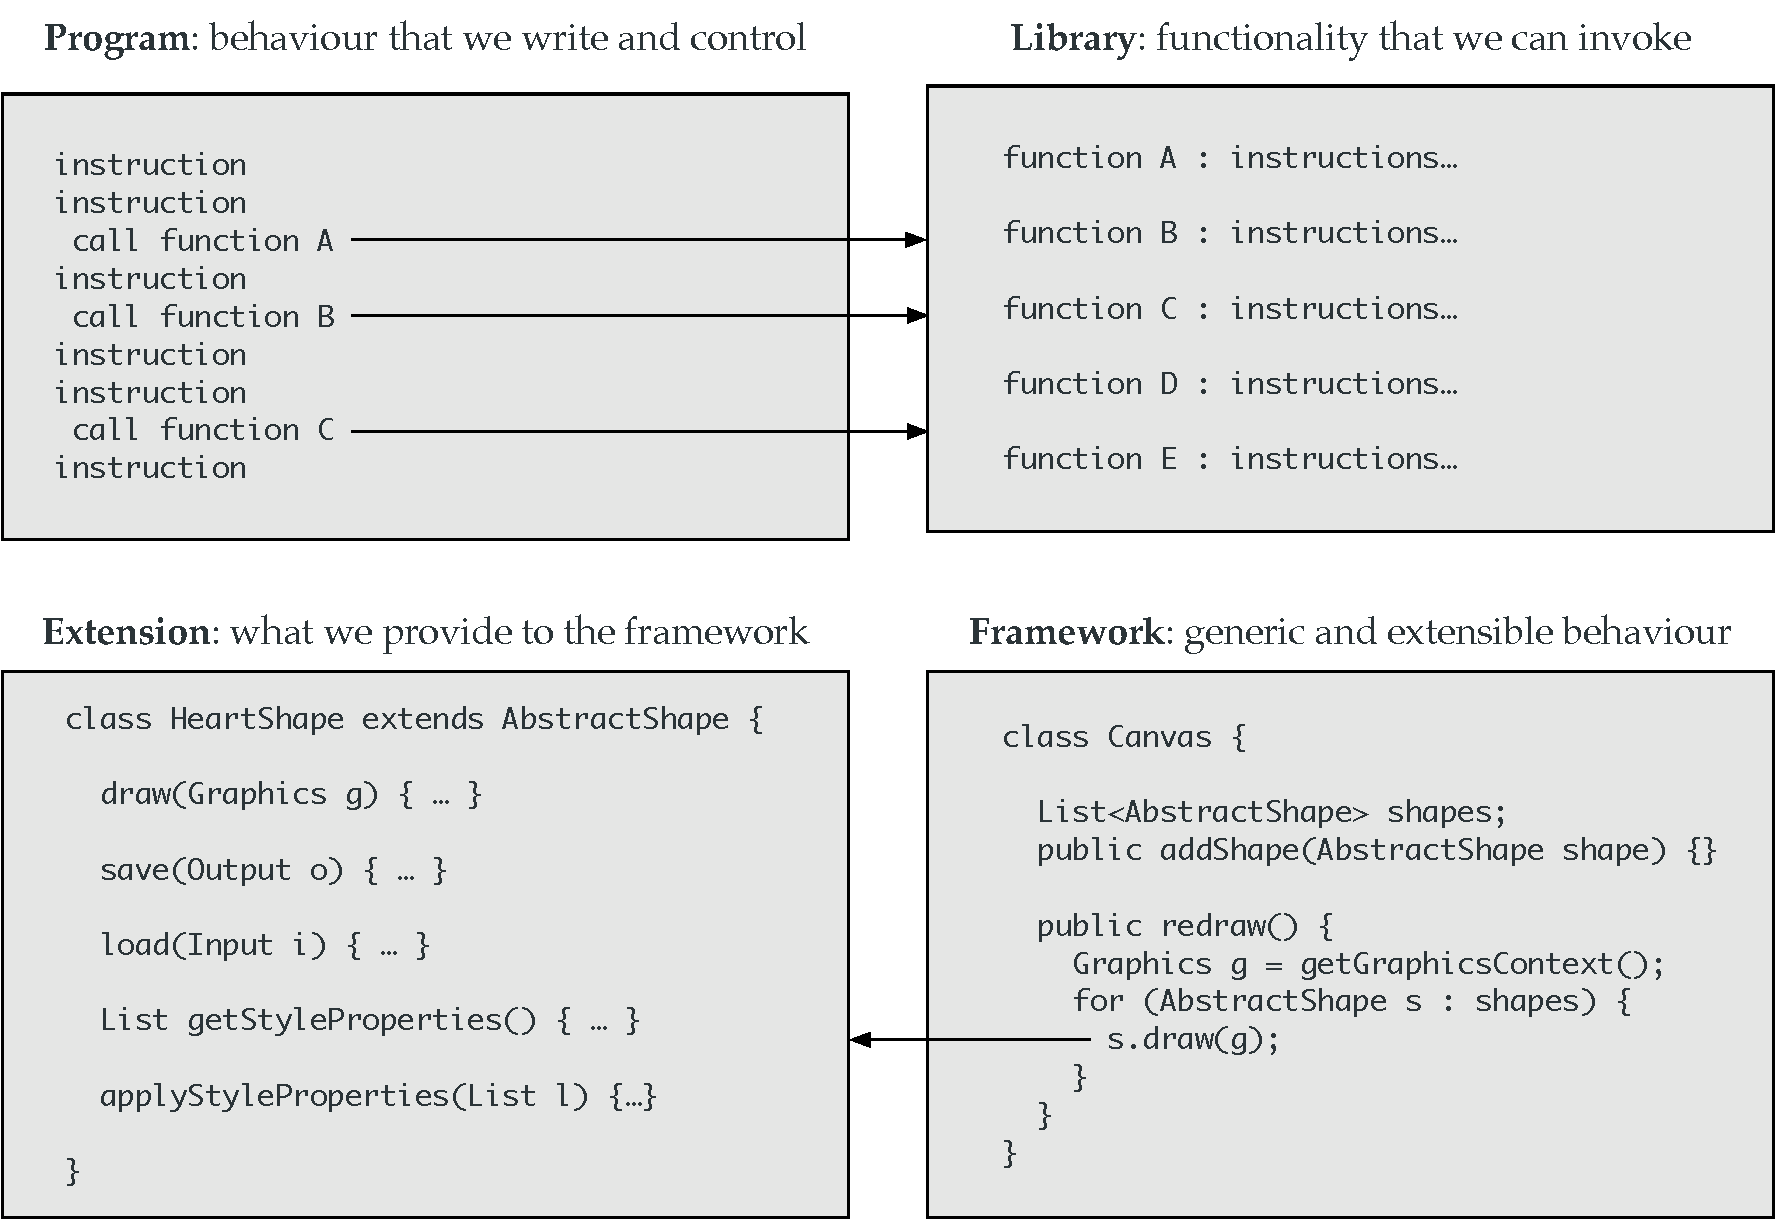
\includegraphics[width=1.0\linewidth]{Figures/frameworkVsLibrary.pdf}
	\caption{Inversion of Control: libraries vs frameworks}
  \label{fig:library-vs-framework}
\end{figure}

\subsection{IoC in the Java EE presentation tier}

As a matter of fact, we have already seen how the \ac{IoC} pattern is applied in the presentation tier, when using servlets.

Let us consider how a developer could build a dynamic web application in Java, but without a Java EE application server. In this case, the developer would use classes from the \texttt{java.net} and \texttt{java.io} packages. He would create a server socket and accept connection requests in a loop. For every new client, he would read the incoming HTTP request line by line. He would prepare a response and send it back to the client, via the socket. Clearly, the developer would control the flow and make calls to classes and methods provided by the Java runtime environment.

The code that we have seen in this chapter follows a different logic. We use the application server as a framework. It implements the generic behavior of any web application: it manages the server socket and accepts client requests. Of course, without us, it is an empty shell and is not able to send meaningful responses to the clients. When we have written the servlet class, we have used an extension point provided by the framework. We have implemented a method that can be called by the application server \emph{at the right time}. But when does the application server decides what is \emph{the right time}? This is where the annotation in Listing \ref{lst:quoteServlet} or the servlet mapping in Listing \ref{lst:quotesProjectDeploymentDescriptor} comes in. The developer uses these mechanisms to register his extension and to specify that it should be called when an incoming HTTP request has certain attributes. The URL is first used to identify the servlet class, the HTTP method is then used to identify the method within this class.

\section{The Pipes and Filters pattern}

The Pipes and Filters pattern can be applied when the processing of a task can be decomposed in a number of steps, and when the steps can be handled by independent, reusable building blocks. The pattern is not specific to multi-tiered applications and can be applied in a wide range of situations. One example is the usage of the \emph{pipe} operator to combine unix commands in a sequence. Another example is the use of the \texttt{Filter} classes in the \texttt{java.io} package, which make it possible to apply different transformations when reading and writing data streams.

\subsection{Description of the pattern}

The pattern is represented in Figure \ref{fig:pipesAndFilters}. The \emph{source} produces a \emph{stream} of \emph{tasks}, which enter a processing \emph{pipeline}. The \emph{pipeline} is not a monolithic piece of code. Instead, it is created by assembling a series of \emph{filters}. Every \emph{filter} performs a well-defined function on the \emph{task}. This means that the \emph{task} can be modified or augmented before being passed to the next \emph{filter}. At the end, the sink receives the result of the computation. The great thing about this pattern is that it is possible to reuse \emph{filters} in different types of \emph{pipelines}. 

\begin{figure}[]
	\centering
    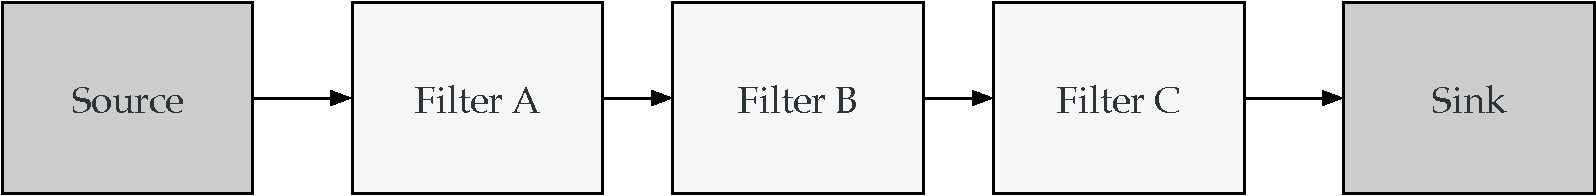
\includegraphics[width=1.0\linewidth]{Figures/pipesAndFilters.pdf}
	\caption{The Pipes and Filters design pattern}
  \label{fig:pipesAndFilters}
\end{figure}

\begin{figure}[]
	\centering
    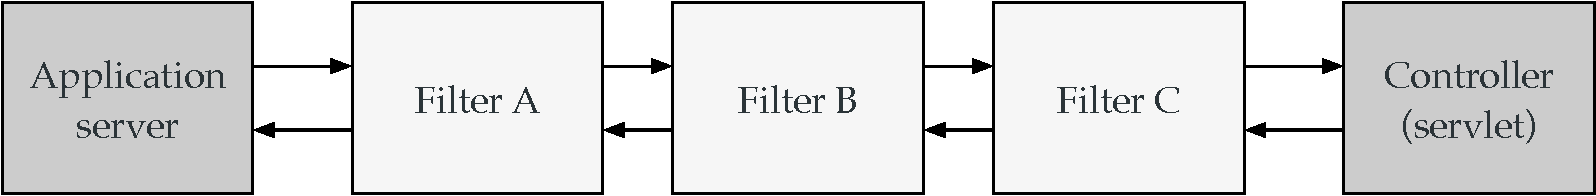
\includegraphics[width=1.0\linewidth]{Figures/pipesAndFiltersHttp.pdf}
	\caption{The Pipes and Filters design pattern in the presentation tier}
  \label{fig:pipesAndFiltersHttp}
\end{figure}

\subsection{Pipes and Filters in the presentation tier}

When applying the pattern in the presentation tier, the tasks processed by the pipeline are the HTTP requests. The application server, which receives the request, is the source. HTTP requests are processed by several filters before they reach the controller. In fact, as shown in Figure \ref{fig:pipesAndFiltersHttp}, the pattern is applied twice: HTTP responses produced by the controller also go through the sequence of filters, which have the opportunity to modify them.

But what is the reason for using filters and what kind of processing is typically done in these components? These are common use cases:

\begin{itemize}
\item \emph{auditing}: a filter can just observe the requests and generate an audit log
\item \emph{authorization}: a filter can decide if the user making the request has the right to do it
\item \emph{compression}: a filter can decompress incoming requests and compress outgoing responses
\item \emph{encryption}: a filter can decrypt requests and encrypt responses
\item \emph{caching}: a filter can optimize performance by reusing previously generated responses (in this case, the filter may short-circuit the pipeline)
\end{itemize}

In order to create custom servlet filters, the developer needs to implement the \texttt{Filter} interface, which defines three methods: \texttt{init(FilterConfig filterConfig)}, \texttt{destroy()} and most importantly \texttt{doFilter(ServletRequest request, ServletResponse response, FilterChain chain)}. An example is shown in Listing \ref{lst:servletFilterExample}. Here are some explanations about the code:

\begin{itemize}
\item line 7: the annotation registers the filter, so that \ac{IoC} can happen
\item line 8: we implement the \texttt{Filter} interface
\item line 12: \texttt{doFilter} is called when the requests advances in the pipeline. Other filters might have been called before, other filters might be called after. The \texttt{chain} parameter represents the processing pipeline.
\item line 19: to test the pipeline, we simply attach a String model to the request. This model will be available in other filters, in the controller servlet and in the \ac{JSP} template.
\item line 21: we pass the request further down the chain.
\item line 23: when the call returns, we have the ability to inspect the response and to modify it. However, if we want to do that, we need to wrap \texttt{resp} in a special object, to capture the output stream in memory.
\end{itemize}

\lstset{
	caption={A servlet filter example},
	language=java,
	label={lst:servletFilterExample}
}
\vspace{10pt}
\begin{minipage}{\linewidth}
\begin{lstlisting}[frame=single]
package ch.heigvd.amt.mvcsimple.presentation;

import javax.servlet.*;
import javax.servlet.annotation.WebFilter;
import java.io.IOException;

@WebFilter(filterName = "CustomFilter", urlPatterns = "/*")
public class CustomFilter implements Filter {
    public void destroy() {
    }

    public void doFilter(ServletRequest req, ServletResponse resp, FilterChain chain) throws ServletException, IOException {
        /*
         The pipeline is first going from the app server towards the controller.
         We can log the request, transform the request. We can also block the 
         request (by not calling chain.doFilter(req, resp);
         */

        req.setAttribute("computedByFilter", "yellow");

        chain.doFilter(req, resp);

        /*
         We are on the way back. Now, we can transform the response. But to
         do that, we would need to send a wrapper to the chain in the previous 
         call. You can find an example in the Java EE 5 tutorial
         */
    }

    public void init(FilterConfig config) throws ServletException {
    }

}
\end{lstlisting}
\end{minipage}

\section{Questions}

To answer these questions, you will need to have read the chapter but also to have done some research. Make sure that you are able to answer every question. Discuss your responses with your peers.

\begin{enumerate}
\item \emph{How does one implement HTML form processing in Java EE?} Consider the scenario where the user arrives on a page, fills out three fields (\texttt{first name}, \texttt{last name} and \texttt{e-mail address}) and presses a \texttt{Register} button. We want to process the event on the server side and to validate the data entered by the user (the fields cannot be empty and the e-mail address must contain an @ sign). What code do you have to write?
\item \emph{What is the difference between the request, session and application scopes in the servlet API?} The method \texttt{setAttribute} is available in the \texttt{HttpServletRequest}, \texttt{HttpSession} and \texttt{ServletContext} classes. What is the difference and when should they be used?
\item \emph{Why do we have to be careful with the \texttt{HttpSession} object?}. The Servlet API makes it very easy to store objects in the session. While it is practical to use this feature to build stateful applications on top of the stateless HTTP protocol, it does not come for free. There are at least risks or drawbacks to be aware of. What are they?
\item \emph{How do we deal with relative links in \ac{JSP} templates?}. It is possible to deploy several applications in the same applications server. For this to work, every application is assigned a \emph{context root}. In order to generate links to CSS files and other assets, it is often necessary to include the context root in the path and it is a bad idea to hard-code the value in the template. What is the solution to this problem?
\end{enumerate}


